% MUST use a4paper option
% MAY use twoside, smaller font, and other class - but not for Självständigt arbete i IT
\documentclass[a4paper,12pt]{article}
% Use UTF-8 encoding in input files
\usepackage[utf8]{inputenc}
% Use T1 font encoding to make the \hyphenation command work with UTF-8
\usepackage[T1]{fontenc}

% Om ni skriver på svenska, använd denna rad:
% \usepackage[english,swedish]{babel}
% If you are writing in English, use the following line INSTEAD of the previous (note order of parameters):
\usepackage[swedish,english]{babel}

%MY OWN PACKAGES
\usepackage{algorithm}
\usepackage{algorithmicx}
\usepackage{algpseudocode}

% Use the template for thesis reports
\usepackage{UppsalaExjobb}

\usepackage{enumitem}
\usepackage{svg}
\usepackage{subcaption}
\usepackage{caption}
\usepackage{mwe}
\usepackage{xr}
\usepackage{xcolor}
\usepackage{listings}
\lstset{language=C,keywordstyle={\bfseries \color{blue}}}

% För att göra ett index behövs
%  - \usepackage{makeidx}
%  - \makeindex i "preamble", dvs före \begin{document}
%  - \printindex, typiskt sist, före \end{document}
% - och att man lägger in \index{ord} på olika ställen i dokumentet
\usepackage{makeidx}
\makeindex


% Designval: per default används styckesindrag, men ibland blir det snyggare/mer lättläst med tomrad mellan stycken. Det åstadkoms av de följande raderna.
% Tycker ni om styckesindrag mera, kommentera bort nästa två rader.
\parskip=0.8em
\parindent=0mm

% Designval: vill ni ha en box runt figurer istället för strecken som är default, av-kommentera raden nedan. Obs att både \floatstyle och \restylefloat behövs.
%\floatstyle{boxed} \restylefloat{figure}

\begin{document}
% För att ställa in parametrar till IEEEtranS/IEEEtranSA behöver detta ligga här (före första \cite).
% Se se IEEEtran/bibtex/IEEEtran_bst_HOWTO.pdf, avsnitt VII, eller sista biten av IEEEtran/bibtex/IEEEexample.bib.
%%%% OBS: här ställer ni t.ex. in hur URLer ska beskrivas.
\bstctlcite{rapport:BSTcontrol}

% Set title, and subtitle if you have one
\title{Partial Compaction in ZGC Using Free-Lists} % och uppsatsmetodik
% Use this if you have a subtitle
%\subtitle{beskrivande men gärna lockande}
%\subtitlesubtitle

% Set author names, separated by "\\ " (don't forget the space, or use newline)
% List authors alphabetically by LAST NAME (unless someone did significantly more/less, which should not be the case)
% For drafts, include your email addresses to make it easier to send peer reviews

\author{Niclas Gärds}

% Visa datum på svenska på förstasidan, även om ni skriver på engelska!
\date{\begin{otherlanguage}{swedish}  %\foreignlanguage doesn't seem to affect \today?
    Juni 2024
  \end{otherlanguage}}

% Använd detta om året för rapporten inte är innevarande år
%\year=2018

% Ange handledare, ämnesgranskare, examinator om dessa finns
\handledare{Erik Österlund}
% There is also \exthandledare
\reviewer{Tobias Wrigstad}
\examinator{Lars-Åke Nordén}

% This creates the title page
\maketitle

% Change to frontmatter style (e.g. roman page numbers)
\frontmatter

%%%% OBS: Läs också källkoden till alla text/X.tex.
%%%% Tips: ni kan använda separata filer för de olika delarna i er rapport på motsvarande sätt,
%%%% men använd inte samma filnamn!

\begin{abstract}
  \input{text/abstract}
\end{abstract}

\begin{sammanfattning}
  \input{text/sammanfattning}
\end{sammanfattning}

% Innehållsförteckningen här.
\tableofcontents

% Här kan man också ha \listoffigures, \listoftables

\cleardoublepage

% Change to main matter style (arabic page numbers, reset page numbers)
\mainmatter

% Here comes the text of the report.

\section{Introduction}
\label{sec:introduction}

%%% Local Variables:
%%% mode: latex
%%% TeX-master: "main"
%%% End:

The most common technique for automatic memory management is garbage collection. The task of a garbage collector is to keep track of which parts of memory are being used by the program which is being executed. Different implementations of garbage collectors offer different benefits over others. The choice of garbage collector heavily impacts the performance and characteristics of the program being executed.

Java is a programming language with dynamic memory management that makes use of garbage collectors to handle memory. Operating within a runtime environment known as the Java Virtual Machine (JVM), Java allows users to configure the JVM to improve performance, including the choice of garbage collector. This thesis explores possible improvements that can be made to the JVM and its garbage collectors. Specifically, the goal is to look at the possibility of implementing a new method for compacting memory in ZGC, one of Java's most recently added garbage collectors.

ZGC stores data in different regions of memory, where every region includes a set of objects that have been allocated by the Java program running. These regions of memory are referred to as pages. During the compaction phase of a garbage collector, the goal is to decrease the amount of fragmented memory in these pages. A common issue with garbage collectors is the presence of fragmented memory. Fragmented memory can occur when previously allocated objects are suddenly not needed by the program. These dead objects then create holes of unused memory that lie between other live objects still used by the Java program. 

In ZGC, a so-called \textit{bump pointer} is used for allocating objects, which offers a fast method of allocating objects, but limits the choice of where to place the objects. To reclaim the unreachable memory, ZGC performs compaction on a page by evacuating all of its live objects into a new empty region, placing them more compactly to get rid of the holes in memory. And if there is no available memory to create an empty page, a more computationally heavy operation will be done to compact all objects into the same page they are currently in. Creating new pages and doing computationally heavy operations to perform compaction are the only two options for ZGC, but with the new method that is explored in this thesis, it is possible to relocate objects straight into the fragmented holes of memory using a free-list based allocator. The benefit of representing memory with free-lists is that it does not limit the available memory to a singular contiguous block of memory like the bump-pointer, instead allowing free memory to be represented by a set of many smaller blocks of memory.

During this thesis, two different free-list based allocators were integrated into ZGC. Both allocators offer the same functionality, but differ in their performance due to their different design choices. J. Sikström and C. Norrbin have both conducted separate thesises on the implementation of a TLSF allocator~\cite{joel} and a Buddy allocator~\cite{casper}, respectively. These allocators were designed by Sikström and Norrbin to meet the requirements of ZGC, and this thesis shows their integration into ZGC to be used for compacting memory. 

\subsection{Purpose and Goals}
\label{sec:purpose}
This thesis evaluates the feasibility and effectiveness of integrating free-list based allocators within ZGC to enhance memory compaction processes and reduce fragmentation. By implementing and benchmarking two distinct allocators, the TLSF and Buddy systems, against the conventional bump-pointer method used by ZGC, this study aims to provide a comparative analysis focusing on key performance metrics including allocation throughput, fragmentation levels, and overall efficiency.

The research examines the trade-offs involved when incorporating free-list allocators into ZGC, such as potential increases in computational overhead and complexity in the allocation process. These factors are quantitatively assessed to offer a balanced perspective on both the advantages and possible drawbacks of this integration.

Furthermore, this thesis explores the broader practical implications and potential applications of free-list based allocators within ZGC and possibly other garbage collectors. Insights gained from this study are expected to guide future research directions, particularly in refining garbage collection techniques and optimizing memory management strategies in Java Virtual Machines.

%%% Local Variables:
%%% mode: latex
%%% TeX-master: "main"
%%% End:


\subsection{Delimitations}
\label{sec:delimitations}
%%% Local Variables:
%%% mode: latex
%%% TeX-master: "main"
%%% End:
This report only covers the integration of a free list allocator in ZGC, and not the implementation of the allocator itself. The integration process assumes that such an allocator is already available, and the project focuses on integrating it into the ZGC code base.

As this project covers the integration of a free list allocator in a large code base, the project is limited to using the free-list based allocator in the compaction phase of the garbage collector when moving live objects. The garbage collector could potentially benefit from using a free-list based allocator for initially allocating objects, but the design of ZGC currently only performs those types of allocations on newly created regions of memory, meaning there are no fragmented holes.

The way ZGC classifies object sizes puts a delimitation on where the new relocation strategy will be applied. In order to get the most variation of the fragmented memory, objects classified as small will be targeted. Most allocations are small and tend to not be allocated for very long. This makes small allocations the prime subject for benefitting the most from constructing free-lists, since their short life span causes memory to get fragmented quicker. Properly evaluating the relocation of small allocations will be a better use of time than implementing the strategy for the other size classes.

Another delimitation to this project is related to how ZGC is a generational garbage collector, meaning it differentiates between \textit{young} and \textit{old} objects. This project will only cover the implementation of compacting young objects since those are the most common types of objects. Due to time constraints, it would be impractical to implement and evaluate the relocation strategy for old objects.

\subsection{Individual Contributions}
\label{sec:individual_contrubitons}
\input{text/individual_contributions}

\paragraph{Acknowledgement}
I would like to thank my supervisor Erik Österlund and subject reviewer Tobias Wrigstad for their fantastic help throughout this thesis project. Their expertise in the subject offered great guidance during the entirety of the project. I would also like to thank the people at Oracle for providing a great workplace environment, where I felt welcome to ask for help at any time.

%%% Local Variables:
%%% mode: latex
%%% TeX-master: "main"
%%% End:


\newpage
\section{Background}
\label{sec:background}
\input{text/background}

\subsection{Memory Management}
\label{sec:memory_management}
\input{text/memory_management}

\subsection{Fragmentation}
\label{sec:fragmentation}
\input{text/fragmentation}

\subsection{Memory Allocation}
\label{sec:memory_allocation}
\input{text/memory_allocation}

\newpage
\subsection{Garbage Collection}
\label{sec:gc}
\input{text/GC}

\subsection{OpenJDK}
\label{sec:openjdk}
\input{text/openjdk}

\subsection{The Z Garbage Collector}
\label{sec:zgc}
\input{text/zgc}

\subsubsection{Pages}
\label{sec:zpage}
\input{text/zpage}

\subsection{Partial Compaction}
\label{sec:partial-compaction}

%%% Local Variables:
%%% mode: latex
%%% TeX-master: "main"
%%% End:

Partial compaction is in the context of memory management the act of compacting a small portion of the heap to decrease the amount of fragmentation in the part of the heap that was compacted. In a paper by A. Bendersky and E. Petrank, it was shown that it is indeed possible to reach lower levels of fragmentation with partial compaction and the use of a free-list based allocator~\cite{partial-compaction}. Using a non-moving allocator, they derive an upper and lower bound to the necessary size of the heap to satisfy the executing program's allocations.

\newpage
\section{Related work}

%%% Local Variables:
%%% mode: latex
%%% TeX-master: "main"
%%% End:

In this section, we review research that has already been done on the subject of ZGC, as well as garbage collection in general. By looking at what has been done previously, the goal is to build up knowledge about what more there is to explore, and how this thesis project will build upon what they have discovered. 

\subsection{ZGC}
As ZGC is the main topic of this thesis, and is the reason this thesis exists, it is only fitting to cover some of the previous research that has been done to improve ZGC. The first paper is one from 2019 about \textit{Improving relocation performance in ZGC by identifying the size of small objects}, written by Jinyu Yu~\cite{zgc:yu}. This paper researched the option of reducing the number of relocations being done for compaction by introducing a new classification for object sizes in ZGC. The results from this paper show that it is a valuable effort to try to reduce the number of relocations being done. With a decrease of about 40\% of all relocations, the throughput stayed unchanged during most benchmarks used for evaluation. This thesis will also explore a new way of relocating objects, but define a new way of representing the relocation destination.

Another paper was written by L. Shoravi, where he explored the option of compressing pointers in ZGC~\cite{zgc:shoravi}. The mission of compressing pointers is to reduce the amount of memory used by the garbage collector. While this thesis does not use compression to reduce the amount of memory used by the garbage collector, the goal is to use memory more efficiently and reduce fragmentation, which is also a way of reducing the total memory used by the garbage collector.

\subsubsection{Other Garbage Collectors}
C. Tauro et. al. wrote a paper on the comparison of two different garbage collectors in Java: CMS and G1~\cite{gc:tauro}. CMS, in contrast to the garbage collector studied in this thesis, ZGC, uses free-lists to represent available memory in the heap. In the paper, they find that CMS performs significantly better in memory usage than what is observed by looking at G1, another regional garbage collector. However, according to their evaluations, G1 performs marginally better regarding throughput. This suggests that they both have benefits that can be desirable when running certain programs. This further motivates the work of this thesis, which is to combine the regional characteristics of ZGC and G1, and the usage of a free-list based allocator like in CMS, and look at what can be achieved when they are used together.

\newpage
\section{Method}
\label{sec:method}

%%% Local Variables:
%%% mode: latex
%%% TeX-master: "main"
%%% End:

\subsection{Integration Method}
% https://ieeexplore.ieee.org/stamp/stamp.jsp?tp=&arnumber=6312870 källa kanske. 1975 LOL

This thesis employs a cyclical development method for integrating a new feature into an existing codebase. The approach is designed to iteratively refine the integration through repeated iterations of evaluation and modification.

\begin{description}
  \item[Phase 1: Analysis]
  The initial phase involves a detailed examination of the system to identify areas impacted by the integration of the new feature. This involves an in-depth review of the existing code, experimental adjustments to observe possible impacts, and consultations with the code's original developers. The purpose of this phase is to gain a comprehensive understanding of the system's functionality and dependencies, which facilitates accurate identification of critical modification points.
  
  \item[Phase 2: Iterative Integration]
  Following the preliminary analysis, the integration ph-ase proceeds in an iterative manner. It begins with creating an implementation design, derived from the insights gained during the analysis phase. The integration then proceeds with applying the planned changes, followed by testing to evaluate the correctness and impact of these changes. If the integration achieves the expected outcomes, the process is completed. If not, the feedback from testing informs further refinements in the plan, and the cycle repeats - designing, implementing, and testing — until the integration fully aligns with the desired functionality, and programs are executed without errors.
\end{description}

This cyclical method offers a systematic approach to implementing new functions in a large code base. By iteratively improving the design, and always making sure to assess the current iterations impacts on the code before moving on to further changes, the final implementation is less prone to fail.

% This project outlines the integration of a new feature in a large code base. New implementations in large code bases tend to have bigger impacts than intended since it is hard to know which parts of the system are going to be impacted. The integration method used during this thesis consists of two different phases, the identification phase, and then the implementation phase. 

% The goal of the first identification phase is to study the behavior of the program in the areas that are going to be impacted. This involves reading the code, changing the code to see the impacts, and also talking to the authors of the code to better understand what implications a small change might have. The goal is that by the end of this phase, enough information will be gathered about the different parts of the system such that it would be easier to identify which parts of the code have to be changed to implement the new feature.

% The second phase involves the process of actually implementing the desired changes. Firstly, a design of the implementation is made from the gathered knowledge of the identification phase. Following this, an iterative method of implementing the design and testing it is done. If the implementation works as intended, the implementation is considered done, and if the implementation does not work as intended, the implementation phase is restarted and a new design has to be made from the knowledge gathered from the failed tests.

\subsection{Exploratory Programming}
The main method for implementing new changes to the JVM code was using exploratory programming. This method implies making changes to the code and seeing what impacts the changes have based on data that is collected from the program. Some tools used to facilitate this process were debuggers and logging tools. In this section, I explain two useful tools that simplify the process of understanding the code.

\subsubsection{Debuggers}
A debugger is a tool that can run your program with an interface to let the developer know the values of certain variables or locations of memory addresses. A useful tool used during this project is the \textit{rr\_debugger}, designed by O'Callahan et al.~\cite{rrdebugger}, which can be used to record and replay a program's execution with deterministic behavior. This makes it possible to view parts of the program at different times. This is very useful in the context of the OpenJDK since the code consists of several hundreds of thousands of lines of code, which makes it easy to have different parts of the system interacting with each other without the developer knowing. Finding which areas in the code are causing the problem is very important for successfully debugging a faulty program, and this is what the debugger is used for.

\subsubsection{Logging}
The Open JDK has access to logging tools that can produce output files with information about the JVM during its runtime~\cite{java:logs}. This is a powerful tool when working with a large code base because it allows for user-friendly interpretation of the execution of code inside the JVM. While debuggers are useful for understanding the code's execution, the logs provide a more summarized explanation of how the code was executed. 

The JVM is already equipped with different types of log outputs, such as logs that display the performance of the garbage collector. By implementing a new allocation strategy, the JVM can be further equipped with useful information about the performance of the free-list allocator. This is used during this thesis to gather valuable insights into the performance of the new allocators.

\newpage
\section{Evaluation Methodology}
\label{sec:evaluation}
In this section, methods used for evaluating the new compaction strategy added to ZGC are explained.

\subsection{Benchmarking With Dacapo}
In order to evaluate the performance of Java running with the new changes to ZGC, a benchmarking framework called Dacapo is used. Dacapo is a well-documented benchmarking tool that aims to simulate real scenarios of Java programs running~\cite{dacapo}. In Table~\ref{table:dacapo_benchmarks} there is a list of the benchmarks used for evaluating the performance of ZGC with the new allocator in place, along with an explanation of what the underlying Java program tries to simulate. The benchmarks are chosen to be representative of different types of programs and to be able to show the performance of ZGC in different scenarios. The benchmarks also differ in allocation sizes, as well as the lifespan of live objects, which makes for good testing of different scenarios that the garbage collector will encounter.

\begin{table}[H]
  \centering
  \begin{tabular}{|l|p{10cm}|}
    \hline
    \textbf{Benchmark} & \textbf{Description} \\ \hline
    \textbf{avrora} & Simulates Java programs for embedded systems or low-power devices. \\ \hline
    \textbf{fop} & Tests the performance of XML to PDF transformation in Java applications. \\ \hline
    \textbf{h2} & Benchmarks database operations like querying and updating in Java. \\ \hline
    \textbf{pmd} & Analyzes Java source code for common programming mistakes and style violations. \\ \hline
    \textbf{sunflow} & Evaluates the performance of Java applications involved in photo-realistic image synthesis and ray tracing. \\ \hline
    \textbf{xalan} & Measures the performance of XSLT transformations in Java. \\ \hline
  \end{tabular}
  \caption{Dacapo benchmarks used for evaluating the performance of ZGC with the new allocator in place. These benchmarks}
  \label{table:dacapo_benchmarks}
\end{table}

\subsubsection{Benchmarking Configurations}
The benchmark programs will be running inside the JVM. The JVM is configurable using JVM-flags, which are decided when starting the JVM and running a program. The JVM-flags used to evaluate the programs, as well as a description of their impact, are shown in Table~\ref{table:jvmflags}.

\begin{table}[H]
  \centering
  \begin{tabular}{|l|p{10cm}|}
    \hline
    \textbf{Flag} & \textbf{Description} \\ \hline
    \textbf{-XX:UseZGC} & Selects ZGC as the garbage collector in the JVM. \\ \hline
    \textbf{-XX:+ZGenerational} & Specifies that the generational version of ZGC should be used. \\ \hline
    \textbf{-Xmx256m} & Sets the maximum heap size to 256 MB. \\ \hline
  \end{tabular}
  \caption{JVM-flags used while running the benchmarks for evaluation.}
  \label{table:jvmflags}
\end{table}

The Dacapo benchmark itself also offers the ability to configure the runtime of the benchmark suite. The configuration flags used for Dacapo is shown in Table~\ref{table:dacapoflags}.


\begin{table}[H]
  \centering
  \begin{tabular}{|l|p{10cm}|}
    \hline
    \textbf{Flag} & \textbf{Description} \\ \hline
    \textbf{-n 100} & Runs 100 iterations of the same program. \\ \hline
    \textbf{-t 1} & Runs the program using one thread only. \\ \hline
    \textbf{--no-pre-iteration-gc} & Disables the automatic GC done before every iteration. \\ \hline
  \end{tabular}
  \caption{Dacapo configuration flags used while running the benchmarks for evaluation.}
  \label{table:dacapoflags}
\end{table}

\subsection{Evaluation Metrics}
To evaluate the performance changes from applying the proposed changes from this thesis, the new version of ZGC will be compared against the reference version of Java running with ZGC. Since the performance of the new changes to ZGC is heavily dependent on which allocator is being used, the evaluation will be done using both allocators to see if any one of them performs better than the other. The metrics used for evaluating the performance of the garbage collector with the new allocator in place are \textbf{Throughput}, \textbf{Fragmentation}, and \textbf{Utilization}. The aim is that these metrics will provide valuable insight into the performance of the allocator from the point of execution time as well as memory usage.

In order to gather information by the program while running, some changes to the code has been made to report information about the free-lists being constructed every garbage collection cycle. The information available from every free-list is presented in Table~\ref{table:gc_logs_fl}.

\begin{table}[H]
  \centering
  \begin{tabular}{|l|l|p{8cm}|}
    \hline
    Metric & Value & Description \\ \hline
    Exhausted & Boolean & Marks a free-list as exhausted if it failed to allocate something inside of it \\ \hline
    Total Memory & Integer & The total amount of free memory that is available in the free-list \\ \hline
    Used Memory & Integer & The amount of memory which was used up by relocations before the GC stopped relocating objects \\ \hline
  \end{tabular}
  \caption{The metrics that are being kept track of for each free-list in ZGC to report on the performance of the free-list allocator.}
  \label{table:gc_logs_fl}
\end{table}

To measure things related to the throughput of the free-lists, the garbage collection cycle itself has been changed to keep track of general information about the different types of relocations being done. Table~\ref{table:gc_logs_throughput} shows the data available from the garbage collection cycle.

\begin{table}[H]
  \centering
  \begin{tabular}{|p{4cm}|l|p{6cm}|}
    \hline
    Metric & Value & Description \\ \hline
    Bump-Pointer Bytes Relocated & Integer & The total amount of bytes relocated using bump-pointers \\ \hline
    Total Bump-Pointer Relocation Time & Integer & The total amount of time ZGC spent performing the relocation operation which resulted in a relocation using a bump-pointer. \\ \hline
    Free-List Bytes Relocated & Integer & The total amount of bytes relocated using free-list destination \\ \hline
    Total Free-List Relocation Time & Integer & The total amount of time ZGC spent performing the relocation operation which resulted in a relocation inside a free-list. \\ \hline
    Total Bytes in Free-Lists & Integer & The total amount of bytes found while initializing all free-lists in a garbage collection cycle. \\ \hline
    Total Time Spent Constructing Free-Lists &  Integer & The total amount of time spent initializing the free-lists in a garbage collection cycle \\ \hline
  \end{tabular}
  \caption{The metrics that are being kept track of by ZGC to report on the throughput of the different relocation methods.}
  \label{table:gc_logs_throughput}
\end{table}

\subsection{Throughput}
Three different types of throughput will be measured with the new implementation. The first throughput is designed to give a valuable insight into how many more operations need to be done when performing relocations using free-lists, instead of using bump-pointers. This will be done by measuring the time it takes for each relocation and then classifying it as being a free-list relocation or not. The throughput will then be represented by how many bytes of memory can be relocated in a given time frame.

Secondly, the execution time of looking up all the holes between live objects in pages is measured. As well as the time it takes, the throughput will also show how much memory the free-list was able to recover. This will once again result in a throughput measured in how many bytes it was able to find in a given time frame.

The third type of throughput will be a more general one which measures the execution time of the entire benchmarking program. The goal of this is to see if there are any noticeable differences in execution time due to more operations, and longer pause times. A good result would be that the execution time has not changed at all, since that would indicate that the more expensive operations of using a free-list is not expensive enough to cause any major performance issues.

\subsection{Fragmentation}
The second metric, fragmentation, will be used as a measurement of how much memory is being fragmented when using the free list allocator. As previous versions of ZGC do not use free lists to represent the free blocks of memory, this metric will only be measured for the versions of ZGC with the new allocator in place. The fragmentation will be measured by looking at how much memory was gathered in the fragmented memory of a page, and comparing that to how much of that memory was utilized by ZGC during relocation.

This metric will show the feasibility of actually performing relocations in free lists constructed from fragmented pages of memory. If the results show us that the fragmented memory between live objects is not deemed viable for allocating into, the fragmentation should increase due to wasted space. However, if allocations are successful in allocating new objects between the live objects in the page, it would be concluded that it is indeed a viable strategy for relocating objects.

A limitation that is done to this measurement of fragmentation is that only pages that have exhausted their available free-list until an allocation has failed will be taken into account. This is because the solution presented in this thesis uses the allocator regionally for every page of memory, which means that it would be hard to define when a page has fragmented memory if it was never determined to be unusable. Pages that get fully exhausted due to failed allocations can classify all of their unused free memory as fragmented since that memory will be unreachable due to new destination pages being chosen as relocation targets.

\subsection{Utilization}
The utilization of the free-list will be measured by looking at how much of the collected memory was used for compaction. This will give insight into whether too little or too much data is being freed for every free-list. If there is a significant amount of memory being freed which is never used as a target location during relocation, it would indicate that too much memory is collected into free-lists, and the method used to determine where to collect free memory from is unfit.

Utilization will also be measured by how much ZGC is utilizing the available free-lists. The measurement will look at the proportions of relocations that are being done using free-lists, compared to the number of relocations being done using bump-pointers. In combination with the first utilization metric, this will provide valuable insight into whether the total amount of relocations is satisfying the amount of available freed space, or if the choice of which pages should initialize a free-list is the problem. 

%%% Local Variables:
%%% mode: latex
%%% TeX-master: "main"
%%% End:

\newpage
\section{Integration}
\label{sec:integration}
%%% Local Variables:
%%% mode: latex
%%% TeX-master: "main"
%%% End:
This section covers the integration process of how the new allocators are used in the ZGC in order to perform allocations in the external fragmentation of pages. This section will also cover the intricacies of ZGC that have guided the design of the implementation. From this point forward, the process of constructing a free list inside the fragmented memory of a page will be referred to as \textit{recycling} that page's memory, since it will turn the previously considered "garbage" memory into usable memory with a free-list allocator.

% \subsection{Intricacies of ZGC}
% As mentioned in Section~\ref*{sec:background}, ZGC is a \textbf{regional}, \textbf{concurrent}, \textbf{generational}, garbage collector. There are various design choices in the ZGC that have made this possible, and these design choices will have to be addressed in order to maintain these properties with a new allocator in place.
% \begin{description}
%          \item[Regional] Since memory is managed regionally using pages in ZGC, the entire available memory can be seen as split up into many small segments of memory. ZGC is heavily based around the regionality of the memory. Relocations and aging is handled on a page-by-page basis, which is a central part of ZGC's design.
%          \item[Generational] ZGC is a generational garbage collector, which means that some allocations are deemed young, and some old. This is done on a regional basis, where every object inside one page are considered to be the same age. The age is determined based on how many GC cycles the page has survived without being relocated due to fragmented memory. Objects in pages which are relocated are moved into pages with one age above the current one, and the pages that are not selected to be relocated will themselves increase their age. With the integration of a new allocator able to recycle already existing pages, the age of the pages will have to be acknowledged to choose which page to relocate to.
%          \item[Concurrent] With the property of being a concurrent garbage collector, ZGC is able to run garbage collection on multiple threads at the same time. When implementing a new allocator, it is important that said allocator will not halt the program by having multiple threads poking at it at the same time. The program must also consider the concurrency of having the garbage collector run concurrently with the mutator threads running the Java program.
% \end{description}

\subsection{Integration Analysis}
To integrate the allocator in certain areas of the code, the first step was to identify during which phases of the garbage collection cycle the free list allocator can be made available. Since the use case of the allocator is for compaction, the relocation phase is studied. In this section, I cover the parts of the garbage collector that were identified as being impacted by the implementation of a new allocator. None of the features explained in this section is implemented during this thesis.

\subsubsection{Determining Where Free-List Should Be Made Available}
\label{sec:analyse-select}
The first step of using free-lists during relocation is to determine where the free-lists are going to be created. To select which pages are deemed viable as recyclable, the behavior of how ZGC treats pages right before the relocation phase of the garbage collection cycle needs to change. As explained before, ZGC uses relocation for compacting pages of memory, and it does this on a page-by-page basis. Each page either gets categorized as a selected page, meaning its objects will be relocated, or as a survivor, meaning its objects will stay in place. 

In Figure \ref{fig:rel_set_selector}, ZGC's way of constructing a relocation set is illustrated. The images show each page as a circular shape, with a gradient color representing the amount of fragmentation. White represents low fragmentation, and therefore many live objects. Red represents high fragmentation, with a smaller amount of live objects. During the first stage of the relocation set selection ZGC iterates over all pages once, and those pages which are filled below a threshold of $25\%$ fragmented memory are chosen as survivors. In Figure~\ref{fig:rel_set_selector2}, the second stage of the relocation set selection has begun. It continues the selection by first sorting all of the pages based on their fragmentation level. After sorting, it selects the first $n$ pages, where $n$ is a number between 0 and the size of the remaining set of pages. The choice of $n$ is done such that after compaction, the garbage collector guarantees a total memory fragmentation of $25\%$, and then categorizes the remaining pages as survivors.

\begin{figure}[H]
      \centering
      \begin{subfigure}[b]{0.6\textwidth}
                \centering
                \includesvg[width=0.6\textwidth]{figures/select_1}
                \caption{The first phase of the relocation set selection. The garbage collector iterates over all pages of memory with liveness data and categorizes them as either survivors or selected for relocation depending on if the amount of live objects inside the page surpasses the compaction limit of ZGC, by default 75\% of the page's memory.}
                \label{fig:rel_set_selector1}
      \end{subfigure}
      \\
      \begin{subfigure}[b]{0.6\textwidth}
                \centering
                \includesvg[width=0.6\textwidth]{figures/select_2}
                \caption{The second phase of the relocation set selection. The pages begin as sorted based on their fragmentation, and then the garbage collector iterates over the pages until it finds enough pages with enough live objects to fit the compaction limit of ZGC.}
                \label{fig:rel_set_selector2}
      \end{subfigure}
      \caption{An illustration of how ZGC selects pages for relocation. The images show differently colored pages based on their fragmentation. Red means high fragmentation, or small amounts of live objects. White means low fragmentation, or large amounts of live objects. The images also show how the pages are categorized before the start of the relocation phase.}
      \label{fig:rel_set_selector}
\end{figure} 

With the new integration of a free-list based allocator, it now opens up the possibility of using the pages categorized as survivors. In the reference version of ZGC, the survivor pages are frozen and cannot perform any more allocations. The fragmented memory inside survivor pages is therefore unreachable. Using free-lists to represent the unused memory inside survivor pages, it would be possible to utilize this once unreachable memory and make it usable again.

\subsubsection{Requirements For Setting Up a Free-List}
\label{sec:analyse-init}
To construct a complete free-list over the fragmented memory in a page, the liveness data should be up to date with the latest garbage collection cycle. After the marking phase of every cycle, the liveness data is updated, and knowledge about where unused memory is located can be deduced by taking the complement of the set of all live objects.

In the reference version of ZGC, the live data is only available during a very limited time before the relocation phase, because the data is reset before the relocation phase starts. This forces ZGC to create the free-lists over fragmented memory before it can be used during the relocation phase.

\subsubsection{Choosing The Free-List As A Relocation Target}
\label{sec:analyse-use}

ZGC performs relocation by iterating through a set of objects, where the object's intended \textit{Age} chooses the target destination of where the object is going to be relocated. The age of an object is determined by the age of the page it previously existed in. There are 16 possible ages that an object can have, listed in Table~\ref{table:zpage_ages}. With a corresponding integer representation, ZGC uses that integer value as an index in an array to access the target page of an object of that age. 

\begin{table}[H]
      \centering
      \begin{tabular}{|l|l|l|l|l|l|l|l|}
                \hline
                \textbf{Name} & Eden & Survivor1 & Survivor2 & Survivor3 & ... & Survivor14 & old \\ \hline
                \textbf{Value} & 0 & 1 & 2 & 3 & ... & 14 & 15 \\ \hline
      \end{tabular}
      \caption{The possible ages of objects in ZGC, and their corresponding integer representation.}
      \label{table:zpage_ages}
\end{table}

The array of target pages starts off empty, and the first objects that require a page of a certain age to relocate to decide when to acquire a target page, updating the target position for objects of that age. If the allocation fails, the target page gets released, and a new target is acquired. The two possible ways of acquiring a target are as explained in the Background section in Section~\ref*{sec:zpage} through allocating a new page, or performing in-place compaction on the page that the object originated from.

\subsection{Implementation}
In this section I cover the changes done to ZGC, and how it enables the garbage collector to perform relocations in free-lists.
\subsubsection{Interfacing the allocators}
As stated before, this thesis will evaluate the performance of two different allocators, a buddy allocator and a TLSF allocator. In order to make use of the allocators, an interface to their implemented code was created to allow ZGC's allocations to use their allocations techniques.

The buddy allocator had 4 different implementations, each with their own benefits, but the one integrated during this thesis was the Binary Tree Buddy allocator, as it was referred to in Norrbin's report~\cite{casper}. The TLSF allocator by Sikström offered one implementation that was fit for use in ZGC~\cite{joel}.

Both these allocators are fit with special characteristics that might not be present in certain allocators. Some constraints that ZGC has forced the allocators to adapt to are listed below:

\begin{description}
    \item[2MB Heap Size] Since the plan is to implement these allocators inside small pages only, the allocators have been designed to be able to handle heap sizes of exactly 2 MB. 
    \item[Minimum allocations of 16 bytes] The smallest object allocations in Java are 16 bytes.
    \item[Allocation alignment at 8 bytes] All objects are aligned to 8 bytes in memory.
    \item[Free arbitrary ranges of memory] In ZGC, liveness data is only made to track live objects, making it impossible to know which objects have actually become unreachable. It is possible to deduce which areas of a page's memory are unused, but you don't know whether it was previously used by one or more objects. In order to solve this, a method of forcibly releasing allocated memory is available in their allocators.
\end{description}

Because of these adaptations, each allocator can overlook the memory of a small page in ZGC without disobeying the rules of ZGC's memory management characteristics.

\subsubsection{Selecting Recyclable Pages}
\label{sec:implement-select}
In order to recycle pages, the garbage collection cycle was changed to include a way of accessing pages during the relocation phase. In this implementation, the pages that are selected to be accessed during the relocation are chosen to be represented by the Survivor pages which have a high amount of live objects in them. This means that all of the fragmented memory that would have previously lived through to the next garbage collection cycle will be made available through free-list allocations.

After pages have been selected, they have to be stored away by the GC as potential targets for relocation. Since relocations are done with respect to the object's age, the pages are stored in a list of lists, where each nested list is accessed using the age of the object. In Algorithm~\ref{alg:select}, a pseudocode example of the process of storing them in the list of lists is shown. Each list can be accessed using an integer between 1-15, representing the age of that page. The lists are guaranteed to include pages that have an available free-list. 

\begin{algorithm}[H]
      \caption{\textproc{init\_free\_list}$(O, T, F)$}
      \label{alg:select}
      \begin{algorithmic}[1]
                \Require 
                \Statex $S$: List of survivor pages.
                \Statex $F$: A list of lists
                \Ensure 
                \Statex $F$ contains all elements of $S$, accessible by the age.
                \ForAll $page \in S$
                      \State $age \gets page_{age}$
                      \State $F[age].append(page)$
                \EndFor
      \end{algorithmic}
\end{algorithm}

In Figure~\ref{fig:generational_free_list_dict} a visual representation of how the pages are rearranged and stored by the GC is shown. The age of each page is shown by their respective integer representation. The age of the page decides which column a page is placed in, and each column represents a set of pages that are available for recycling.

\begin{figure}[H]
      \centering
      \includesvg[width=0.8\textwidth]{figures/select}
      \caption{A visual representation of how the recycled pages are stored by the garbage collector. The pages are stored in a 2-dimensional array, where the column is the age of the page, and each page in that column represents a set of pages that are available for recycling.}
      \label{fig:generational_free_list_dict}
\end{figure}

\subsubsection{Initializing the Free List}
\label{sec:implement-init}
For an allocator to be made aware of the available fragmented memory that is going to be utilized for compaction, the free-list first has to be initialized. The implementation was made such that every single page has a separate allocator, which means that the allocators themselves only overlook the memory of one page. Because of the limitation of only implementing free-lists for small pages, this region is always of size $2$MB.

To construct the free list, all the currently live objects in the page must be taken into account. To map out the areas of free memory the page traverses through all of its live objects and if there is any space between the object which is not allocated, the memory will be acknowledged as free for the allocator. In Algorithm~\ref{alg:init}, the process of creating the free list from the live map is explained with pseudo-code. For every call to the function $free\_range$, a new segment of free memory will be made available in the allocator. 

\begin{algorithm}[H]{}
      \caption{\textproc{init\_free\_list}$(A,R,L)$}
      \label{alg:init}
      \begin{algorithmic}[1]
                \Require 
                \Statex $A$: An allocator.
                \Statex $R$: A region of memory.
                \Statex $L$: A livemap of live objects in a page, ordered by position in memory. Each entry in the live map corresponds to a pointer inside of region $R$. 
                \Ensure 
                \Statex $A$ has complete knowledge of all available blocks of free memory within $R$.
                \State $A.fill()$ \Comment{Start off with fully allocated page}
                \State $curr\gets R_{start}$ \Comment{Start at the beginning of the page}
                \ForAll{$l \in L$}
                \If{$l_{start} - curr \geq 16$}  \Comment{Check if there is a gap between live objects}
                \State $A$.free\_range$(curr, l_{start})$ \Comment{Mark the gap as free}
                \EndIf
                \State $curr\gets l_{start} + l_{size}$ \Comment{Jump forwards to next potential gap in memory}
                \EndFor
                \State $A$.free\_range$(curr,R_{end})$ \Comment{Mark the last memory segment of the page as free}
      \end{algorithmic}
\end{algorithm}

This initialization process is done every garbage collection cycle for every allocator in a survivor page. This was done to avoid issues with pages being used for in-place compaction, which would rearrange all the live objects in the page, desynchronizing the allocation data in the allocator with the actual position of live objects. It would be possible to solve this issue by only recreating the free-list of pages that have performed in-place compactions in earlier cycles, but there is a bonus of updating the free-list every cycle. If the free-list is updated, you can increase the size of the free-list because of new liveness data that can tell if previous allocations have died.

\subsubsection{Using the Allocator}
\label{sec:implement-use}
The goal is not to replace the already existing method of choosing a target page for relocation, but to add to it the ability to choose survivor pages as targets. The implementation of this during the relocation phase is heavily based on the method used for deciding which page is used for relocating objects using bump-pointers, explained in Section~\ref{sec:analyse-use}. The new method allows the option of choosing a target location that is represented by a free-list. The pages that can be chosen as targets are the same as are explained in Section~\ref{sec:implement-select} to have been stored by the garbage collector in a list of lists. 

In Algorithm~\ref{alg:use}, a pseudo-code example of how target pages are chosen, and how the new addition of free-lists are used. Rows 6-10 describe the process of choosing a page with a free-list as a target. This implementation implies that a failed allocation deems the page as unusable, and will discard the free space that may be available there, and claim another page as its target location.

\begin{algorithm}[H]
      \caption{\textproc{init\_free\_list}$(O, T, F)$}
      \label{alg:use}
      \begin{algorithmic}[1]
                \Require 
                \Statex $object$: An object to be relocated.
                \Statex $T$: An array of target pages to relocate objects to.
                \Statex $F$: A list of lists. Each nested list contains pages that have free-lists available to use for allocation.
                \Ensure 
                \Statex $object$ is relocated to a target page stored in $T[object_{age}]$ 
                \State $age \gets object_{age}$
                \State $size \gets object_{size}$
                \State $target \gets T[age]$
                \State $address = target.allocate(size)$
                \If{$address$ not valid} \Comment{$object$ cannot relocate to $target$}
                      \Statex \textbf{Find a new page to relocate the object to. Look for pages with available free-lists.}
                      \State $target \gets F[age].pop()$
                      \If{$target$ is valid}
                              \State $T[age] \gets target$
                              \State $\textbf{GOTO 4:}$
                      \EndIf
                      \Statex \textbf{No free-lists were found to relocate to, resort to allocating a new page and use a bump-pointer for relocating $object$}
                      \State $target = allocate\_new\_page()$ 
                      \If{$target$ is valid} 
                              \State $T[age] \gets target$
                              \State $\textbf{GOTO 4:}$
                      \EndIf
                      \Statex \textbf{Valid $target$ could not be found, must resort to in-place compaction of the page where the object originated from.}
                      \State $T[age] \gets in\_place\_compaction(O_{page})$
                \EndIf
                \State $\text{return successfully}$
      \end{algorithmic}
\end{algorithm}

% The pages are claimed by the thread that is performing the relocation based on which age the object being relocated is. If the relocated object is of age \textit{Eden}, the target age would be one higher than that, \textit{Survivor1}, and so the target page would be chosen from the column that corresponds to that age. In order to stop contention, the page is claimed atomically, which guarantees that no other thread will use the same page as a target location for relocating objects.

% Once a page's free-list is full, and returns an invalid pointer from an allocation call, the garbage collector claims another page and repeats the process until there are no more page's available with a free-list. When there is no available page with a free-list, the garbage collector detects that it is no longer possible to perform the relocation using free-lists, and instead resorts to allocating new pages and use bump-pointer allocations for compacting the rest of the objects that need to be relocated. 

\newpage
\section{Results}
\label{sec:results}

%%% Local Variables:
%%% mode: latex
%%% TeX-master: "main"
%%% End:
This section covers the results of running the new version of ZGC with different types of allocators, comparing them to the reference version of ZGC without the applied changes. The results both display the allocator's performance of utilizing the fragmented memory with a free-list representation, as well as the garbage collector's ability to utilize these allocators.

\subsection{Free List Performance}
In this section, the performance of the new memory allocator is assessed based on its allocation throughput, initialization throughput of the free list, and the measured fragmentation at the time of a free-list being exhausted.

\subsubsection{Allocation Throughput}
For the allocation throughput, Figure~\ref*{fig:allocation-throughput} shows the results for the different implementations while running six different benchmarking programs. The results show us that the cost of relocating the objects using the new free-list allocator is not that big. The bump-pointer exceeds the throughput of the free-list allocators in always every benchmark, except for one, Sunflow, where the throughput of the Buddy allocator is the fastest. This tells us that the overhead operations of finding which destination page to perform a relocation into might outweigh the operation of allocating objects with a free-list allocator, which is a positive result that implies 

\begin{figure}[H]
\centering
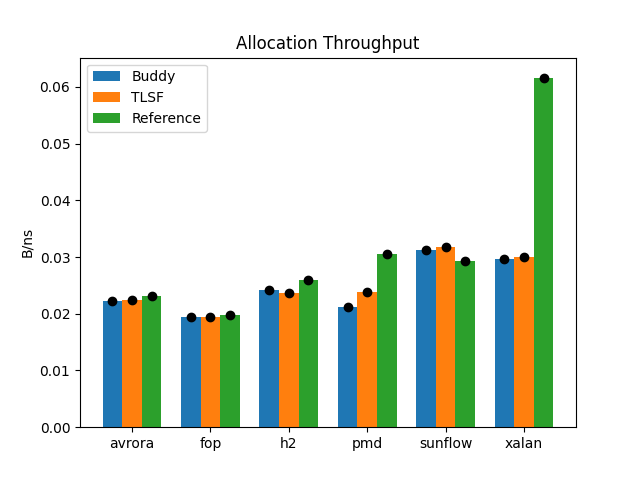
\includegraphics[width=1\textwidth]{figures/allocation_throughput2.png}
\caption{Barplot showing the allocation throughput of the different allocation strategies when performing relocations.}
\label{fig:allocation-throughput}
\end{figure}

\subsubsection{Free List Initialization Throughput}

To measure the cost of searching for the free memory in the fragmented memory of a page, the initialization process of the free-list was introduced. Results shown in Figure~\ref{fig:free-list-initialization} show the throughput you get from initializing the free list. The numbers displayed show us that there is a significant cost to initializing the free list. Important to note here is that the difference in throughput between each of the benchmarks is because of the allocation patterns of the programs, and not a variation in the performance of the machine running the program. 

\begin{figure}[H]
\centering
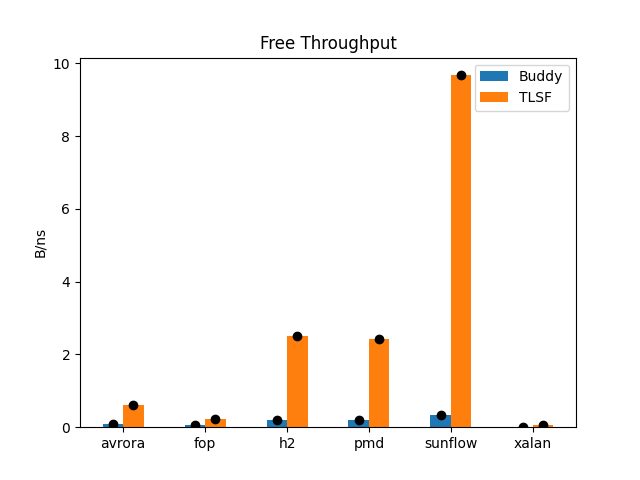
\includegraphics[width=1\textwidth]{figures/free_throughput2.png}
\caption{Barplot displaying the throughput of adding bytes of free memory to the allocator's free-list. The throughput is calculated as the amount of bytes found in the fragmented memory, divided by the time it took to execute the initialization process.}
\label{fig:free-list-initialization}
\end{figure}

\subsubsection{Fragmentation}
\label{sec:results:frag}
The different allocators demonstrate a significant difference in their ability to make use of the available memory, displaying some huge variations in how much memory can be claimed before an allocation is too large to handle. This is evident from Figure~\ref*{fig:memory-fragmentation}. The plot shows different results for different benchmarking programs, but the TLSF allocator performs significantly better on all benchmarks.

\begin{figure}[H]
\centering
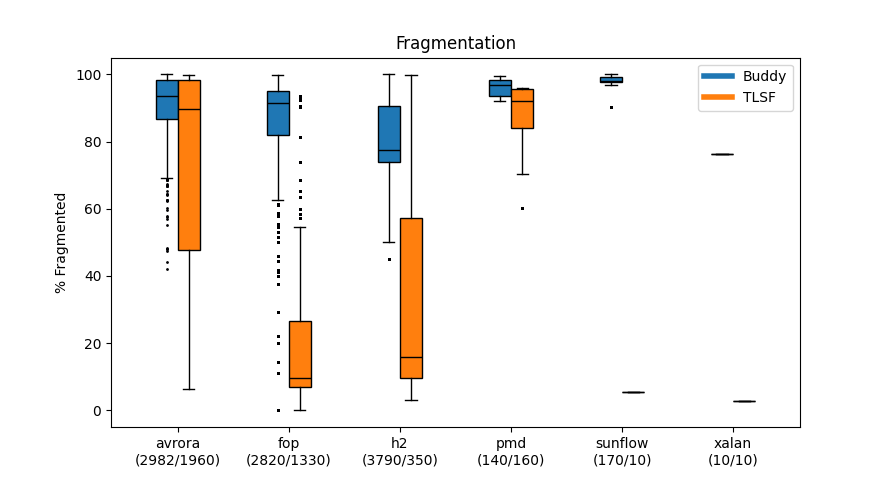
\includegraphics[width=1\textwidth]{figures/fl_fragmentation2.png}
\caption{Boxplots for each benchmark, and different boxplots for the two implementations measured. Each measured data point is taken from the set of exhausted pages from a full run of the specified benchmark. The fragmentation is measured as the amount of used up bytes, divided by the total amount of bytes available. The numbers displayed by the benchmark name denote the amount of data points measured for each implementation.}
\label{fig:memory-fragmentation}
\end{figure}

\subsection{Benchmark Performance}
This section evaluates the garbage collector's performance across various benchmarks, focusing on the Java program in its entirety while running with the new implementation of ZGC using free list allocators and comparing that to the reference version of ZGC on which the new implementation was built.


\subsubsection{Relocation Duration}

Although overall execution time remains stable, there's a marginal increase in the time that the garbage collector spends in the relocation phase. In Figure~\ref{fig:relocation-duration}, the relocation duration over multiple runs is shown. It is possible to see a slight upward trend in relocation time for the implementations using free-list relocations. 

\begin{figure}[H]
\centering
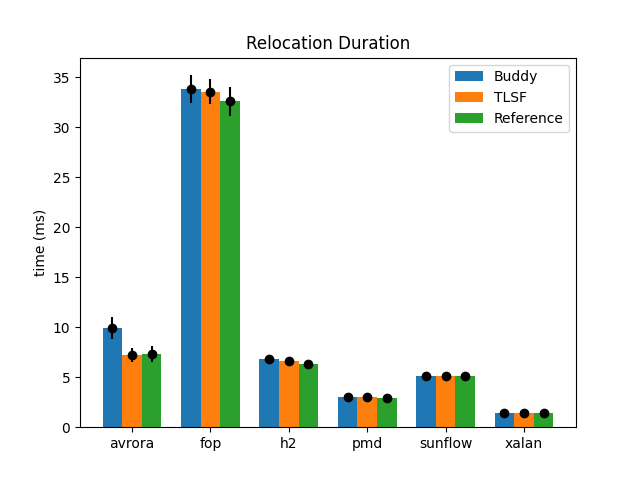
\includegraphics[width=1\textwidth]{figures/relocation2.png}
\caption{Barplot showing the average duration that the garbage collector spent in the relocation phase. The reference version only uses bump pointer allocations, while the buddy allocator and TLSF allocator make use of a free-list allocation method, but resort to bump pointers when needed.}
\label{fig:relocation-duration}
\end{figure}

\subsubsection{Relocation Set Selection Duration}

This metric shows the time it takes for the garbage collector to select which pages are going to be used for relocation, which is the phase impacted by the initialization of free list memory. In Figure~\ref{fig:set-selection}, a barplot shows the average time that the different implementations spend in the relocation set selection phase of the garbage collection cycle.

\begin{figure}[H]
\centering
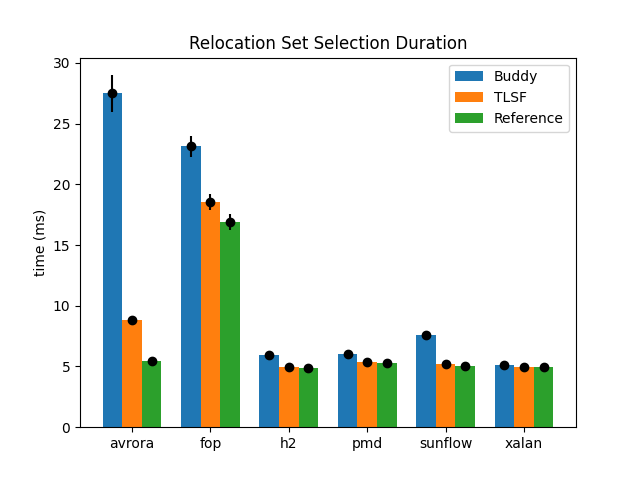
\includegraphics[width=1\textwidth]{figures/set_selection2.png}
\caption{Barplot showing the average Relocation Set Selection duration across six different benchmarks.}
\label{fig:set-selection}
\end{figure}


\subsubsection{Throughput}
In Figure~\ref{fig:execution-time}, the relative execution times are displayed from running the six different benchmarks for 250 iterations each, comparing the three different implementations. Across the multiple executions of the benchmark, the execution time remains largely consistent across all implementations, with overlapping standard deviations from the average. 

\begin{figure}[H]
  \centering
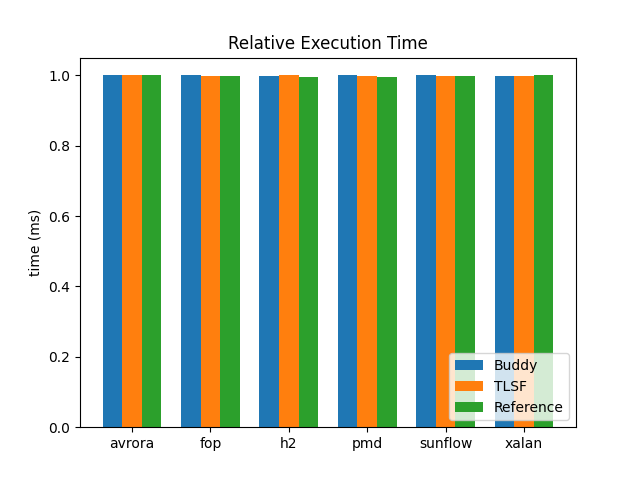
\includegraphics[width=1\textwidth]{figures/execution_time2.png}
\caption{Boxplot of the measured throughput in terms of execution time. The times are normalized to a value between 0 and 1, where the implementation with the longest execution time is set to 1, and the other are shown as a smaller or equal proportion of that.}
\label{fig:execution-time}
\end{figure}

\subsubsection{Utilization}
The utilization metric is measured in two different ways. First by looking at how much of the free-list memory is being used up by the GC every cycle. Also, the GC's capability of utilizing free-list memory is measured by looking at the proportions of relocations that are done using free-lists, compared to using bump-pointers.

In Figure~\ref{fig:utilization}, a bar plot is shown displaying the results from the six different benchmarks, and their ability to use the free-list memory. Except for the benchmarking program \textit{fop}, the average utilization of free-list memory is around 1\%, meaning there is a lot more memory that is being freed than is necessary.

The utilization of free-lists in the relocations phase was also measured, and the results can be seen in Figure~\ref*{fig:relocation-utilization}. The bar plot displays the average amount of relocations that were done using free-lists, instead of bump-pointers. 

\begin{figure}[H]
  \centering
  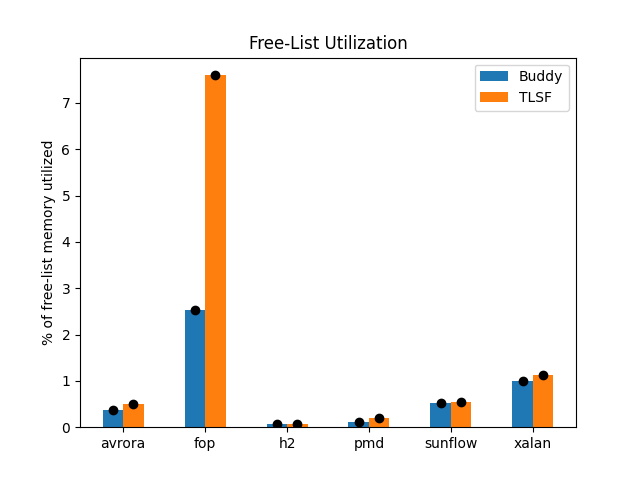
\includegraphics[width=1\textwidth]{figures/utilization2.png}
  \caption{Barplot showing the utilization of free-list memory in benchmarks, measured by dividing the allocated memory in the free-list by the size of the entire free-list.}
  \label{fig:utilization}
\end{figure}

\begin{figure}[H]
  \centering
  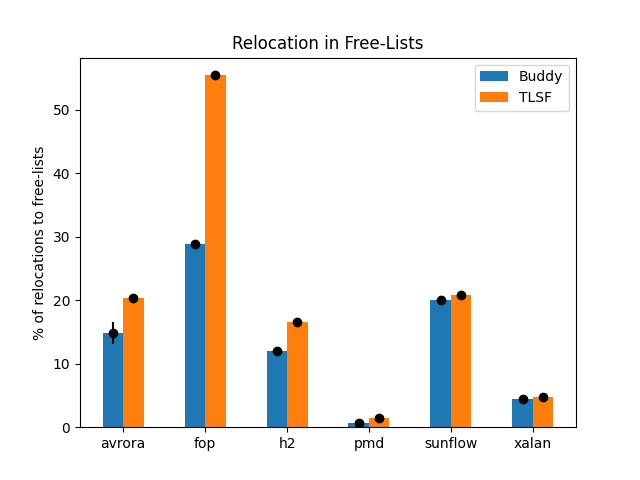
\includegraphics[width=1\textwidth]{figures/relocation_utilization2.png}
  \caption{Barplot showing the number of relocations that were done using free-lists, instead of resorting to bump-pointers.} 
  \label{fig:relocation-utilization}
\end{figure}

\newpage
\section{Discussion}
\label{sec:discussion}

In this section, the results are discussed from the context of the purpose and goals which were set at the beginning of the project. 

\subsection{Discussing the Results}
The results from this thesis show us that the new allocators do not add any significant execution time that decreases the performance of the garbage collector, which is a good sign. Results also show that there is indeed an increased amount of operations being done when the free-list allocator is being used. However, the difference is not large enough to cause any performance issues for the Java program being executed. 

Another positive result is that some benchmarks used for evaluating the performance displayed good signs of utilizing the fragmented memory for compaction. The benchmark \textit{fop} performed relocations of objects that were able to use very much of the memory that was found in free-list as a location to compact objects into. With an average fragmentation of approximately 10\% when using the TLSF allocator, it shows us that the fragmented memory between objects is indeed usable. 

The fact that the execution time does not change is a good result in the sense that the expectation was to have a more computationally heavy allocation method, with the upside of being able to utilize memory more efficiently. The results also prove that the fragmented memory was indeed being utilized quite efficiently. However, these results could suggest that the allocator is not doing as much work as expected. The results from this thesis do not tell us enough about the behavior of the garbage collector to know if the amount of memory that was saved from using the fragmented memory was enough to cause any performance increases. Rather, the results hint towards the opposite that the memory saved is not enough to significantly change the performance of the program.

From the results about utilization, there is a noticeable problem. A very large amount of the free-list memory that is created every garbage collection cycle is never used. This is largely because of the method used to choose which pages should construct a free-list, because it currently does not try to balance the relocation set size with the amount of free space in the rest of the pages. However, the problem is not only due to the relocation set size but also the distribution of objects of different ages. Since the age of an object is page-dependent, a free-list can only contain objects of one unique age. It could be the case that free-lists are constructed for a target age that has no relocated objects, meaning the method for selecting a relocation set is unfit for utilizing the full potential of free-lists. 

\subsection{Discussing the Evaluation Method}
The method used for evaluating the performance of the free-lists provided valuable insights into how ZGC behaved with and without the presence of a free-list allocator. The difference between the two allocators, about the reference version of ZGC was also noticed to have an impact on certain metrics, which was one of the goals of evaluating both allocators.

While the choice of benchmarking programs did provide unique relocation patterns that display different performances under different conditions, there are certain issues with how the performance measurements were gathered. The main problem was that some programs did not have enough data points to be able to draw any conclusions. For example, \textit{xalan} from the Dacapo benchmark did not utilize the free-lists nearly as much as \textit{avrora}, as can be seen in Section~\ref{sec:results:frag} on Figure~\ref{fig:memory-fragmentation}, from the small amount of data points in the boxplot. The reason for this is that \textit{xalan} is a program that uses very little memory and does not create a lot of fragmentation when executing inside of the JVM with the chosen configurations. This makes it an unfit program for evaluating the usage of free-lists, since it does not impact the execution of the program much at all. By more thoughtfully picking out benchmarking programs, more valuable data could be gathered about the free-list utilization.

%%% Local Variables:
%%% mode: latex
%%% TeX-master: "main"
%%% End:


\newpage
\section{Future Work}
\label{sec:future}
This thesis has presented a version of ZGC that offers the possibility of utilizing fragmented memory using free-lists. While this implementation has proved that it is possible to perform relocations using free-lists, there is a lot of work that has to be done to reach the full potential of this new relocation technique. This section proposes some future work that could lead to improvements in the utilization of free-lists. Also proposed in this section are some recommended future work that aims to solve problems with the solution presented in this thesis.

\subsection{Potential Future Work}
In the HotSpot VM, the current minimum size of an object is 16 bytes, which forces objects smaller than this to use more memory than necessary. This results in internal fragmentation, which allocates more memory than the program needs. In parallel to this thesis, a project called \textit{Lilliput} is being pursued, which explores the possibility of decreasing the minimum size of objects to 8 bytes from 16~\cite{lilliput}. While this will automatically lower the total amount of memory used by Java programs, it could also prove beneficial when using free-lists. By allowing free-lists to be represented by an even higher degree of granularity, a larger amount of fragmented memory can be represented by the blocks in the free-list.

An additional path worth exploring is to look into the possibility of handling the age of objects on a per-object basis, such that the object itself can tell how old it is, and not base it on the age of the page that it is in. For every object in the HotSpot VM, a 32-bit header of metadata is allocated called the \textit{markword}. The markword contains 4 bits that ZGC currently does not make use of. 4 bits can represent $2^4 = 16$ different states, the same as the amount of different ages that objects can have in ZGC. In the current version of ZGC, mutator allocations would not benefit from utilizing free-lists. This is because no objects of the initial \textit{eden} age are ever determined to be garbage until the first GC cycle, and hence there cannot exist a free-list representation of any fragmented memory. By allowing \textit{eden} objects to exist with objects of other ages, mutator allocations could be done in memory with existing fragmentation, and could potentially allow for the use of free-lists in a new scenario.

\subsection{Recommended Future Work}
The work done in this thesis has not changed how ZGC chooses the relocation set. Pages are chosen to be part of the relocation set depending on the number of live objects that need to be evacuated, which is how ZGC reclaims the fragmented memory in that page. This method of choosing the relocation set is based on the fact that the unused data in pages was not reachable, and could only be utilized by evacuating the entire page. The introduction of a free-list changes this assumption, and opens up the possibility of using the memory without evacuating the page. From the results of this thesis, we can see that the relocation set that is selected is not fit for this use, since the amount of memory represented by free-lists overshoots the size of the relocation set by a lot. By predicting the size of the relocation set, and how much memory is being relocated for each age, free-lists can be constructed to better match the size of the relocation set. This way, ZGC would avoid spending as much time constructing free-lists that will never be used.

Another way forward is to design a high-level allocator that can represent a free-list across multiple pages. In this thesis, the allocators are used on a per-page basis. If an allocator fails to allocate an object, the page is deemed exhausted and the free-list of that page becomes unusable. From the results of this thesis, it could be seen that some benchmarking programs struggled with fragmentation in exhausted free-lists. With the use of a high-level allocator that can combine all pages into a single large free-list, it would not be necessary to exhaust pages to start using another page's free-list, reducing the fragmentation caused by failed allocations.

%%% Local Variables:
%%% mode: latex
%%% TeX-master: "main"
%%% End:


\newpage
\section{Conclusions}
\label{sec:conclusions}


%%% Local Variables:
%%% mode: latex
%%% TeX-master: "main"
%%% End:
This thesis has explored the integration of free-list based allocators within the Z Garbage Collector (ZGC) to better utilize fragmented memory in Java's garbage collection process. The modifications introduced aim to optimize memory management by reallocating fragmented spaces more efficiently, which could lead to enhancements in both garbage collection performance and overall memory utilization.

Key findings include:
\begin{enumerate}
  \item Feasibility of Free-List Integration: The integration of free-list based allocators within ZGC demonstrates that fragmented memory can be effectively reused. This approach helps mitigate the limitations associated with ZGC's traditional bump-pointer allocation method, which often leaves free memory areas unused.
  \item Performance Impact: The implementation maintains comparable performance with the traditional methods under certain conditions, without significant degradation. This shows that utilizing free-lists for memory compaction is a practical approach that does not adversely affect the garbage collector's throughput.
  \item Challenges in Utilization: A significant challenge identified is the underutilization of generated free-lists due to the current method ZGC uses to select relocation sets. This finding suggests that while the theoretical model is sound, practical implementation requires careful consideration of how memory is allocated and reclaimed during the garbage collection cycles.
\end{enumerate}
Overall, the study confirms that employing free-lists within ZGC is a promising strategy for enhancing Java's memory management by reducing fragmentation and making better use of available memory. Further refinement and optimization could lead to substantial improvements in the efficiency and performance of garbage collection processes in JVMs.

%%%% Referenser - SE OCKÅ APPENDIX

% Use one of these:
%   IEEEtranS gives numbered references like [42] sorted by author,
%   IEEEtranSA gives ``alpha''-style references like [Lam81] (also sorted by author)
\bibliographystyle{IEEEtranS}
%\bibliographystyle{IEEEtranSA}

% Here comes the bibliography/references.
% För att göra inställningar för IEEEtranS/SA kan man använda ett speciellt bibtex-entry @IEEEtranBSTCTL,
% se IEEEtran/bibtex/IEEEtran_bst_HOWTO.pdf, avsnitt VII, eller sista biten av IEEEtran/bibtex/IEEEexample.bib.
\newpage
\bibliography{bibconfig,refs}
%\bibliography{refs}

\newpage
\appendix %%%% markerar att resten är appendixar
%%%% I er egen version, ta bort allt nedan (utom \end{document})
\input{text/appendix}

% Om ni har ett index
\makeatletter
\renewenvironment{theindex}
{\if@twocolumn
    \@restonecolfalse
  \else
    \@restonecoltrue
  \fi
  \twocolumn[\section{\indexname}]%
  \@mkboth{\MakeUppercase\indexname}%
  {\MakeUppercase\indexname}%
  \thispagestyle{plain}\parindent\z@
  \parskip\z@ \@plus .3\p@\relax
  \columnseprule \z@
  \columnsep 35\p@
  \let\item\@idxitem}
{\if@restonecol\onecolumn\else\clearpage\fi}
\makeatother
\printindex
\end{document}
